\newcommand{\deadline}{09.06.2023}

\documentclass[11pt, german]{article}

\usepackage[exercise,exp]{custom_2.0}

\begin{document}

\section{Driftgeschwindigkeit im Kupfer}
\subsection{}
\begin{align*}
    j &= nqv\\
    v &= \frac{j}{nq} = \frac{I}{A n q }\\
    n &= n_A N_{frei} \frac{\rho_V}{\rho_n}\\
    v &=  \frac{I\rho_n}{\pi r^2 q n_A N_{frei} \rho_V }\\
    &\approx \frac{500\u{mA}\cdot63.5\ufrac{g}{mol}}{\pi \cdot \frac{1}{2^2} \u{mm^2} \cdot (\chargeelec)\cdot\avogadro \cdot 1 \cdot 8.92\ufrac{g}{cm^3} }\\
    &\approx -4.70\cdot 10^{-5}\ufrac m s = -47.0 \ufrac{\mu m}s
\end{align*}

\subsection{}
\begin{align*}
    j &= n q  v\\
    \sigma_{el} E &= n q a \tau_s\\
    \frac{1}{\varrho_s}E &= n q \frac{qE}{m_e}\tau_s\\
    \tau_s &= \frac{m_e }{\varrho_s n q^2}\\
    &= \frac{m_e \rho_n}{\varrho_s n_A N_{frei} \rho_V q^2}\\
    &\approx \frac{\masselec \cdot 63.5 \ufrac{g}{mol}}
    {1.7\cdot 10^{-8}\Omega\u m \cdot \avogadro \cdot 1 \cdot 8.92 \ufrac{g}{cm^3}(\chargeelec)^2}\\
    &\approx 2.47\cdot 10^{-14}\u s\\
\end{align*}
\begin{align*}
    \Lambda &= v \tau_s\\
     \\
    \frac 12 m v^2 &= \frac{3}{2}k_B T\\
    v &= \sqrt{\frac{3k_B T}{m_e}} \\
    \\
    \Lambda &= \tau_s \sqrt{\frac{3k_B T}{m_e}}\\
    &\approx  2.47\cdot 10^{-14}\u s \cdot \sqrt{\frac{3\cdot \boltzmann\cdot 300^\circ \u K}{\masselec}}\\
    &\approx 2.89 \u{nm}
\end{align*}

\section{Innenwiderstand einer Batterie}
\subsection{}
\begin{figure}[h]
    \centering
    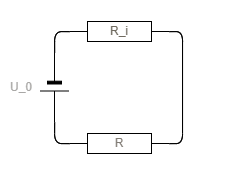
\includegraphics[width=0.4\textwidth]{battery}
    \caption{Schaltbild einer vereinfachten Batterie}
\end{figure}

\subsection{}
\begin{align*}
    -I_0 &= I\\
    -\frac{U_0}{R_{ges}} &= \frac{U}{R}\\
    U &= -U_0 \frac{R}{R_{ges}} \with R_{ges} = R + R_i\\
    I &=  -\frac{U_0}{R_{ges}}\\
\end{align*}

\subsection{}
\begin{align*}
    P &= U \cdot I = R \hug{\frac{U_0}{R_{ges}}}^2 \\
    \\
    \abs{\frac U {U_0}} &= \frac{R}{R_{ges}}\\
    R &= \abs{\frac U {U_0}} R_{ges}\\
    \\
    P &= \abs{\frac U {U_0}} \frac{U_0^2}{R_{ges}} = 0.85\% \frac{U_0^2}{R_i + R} 
\end{align*}

\subsection{}
\begin{align*}
    \rightarrow&\begin{cases}
        U_1 = -U_0 \frac{R_1}{R_{ges}} = -U_0 \frac{R_1}{R_i + R_1}\\
        I_1 = -\frac{U_0}{R_{ges}} = -\frac{U_0}{R_i + R_1}\\
        U_2 = -U_0 \frac{R_2}{R_i + R_2}\\
        I_2 = -\frac{U_0}{R_i + R_2}\\
    \end{cases}\\
    \rightarrow&\begin{cases}
        \frac{U_1}{I_1} = R_1\\
        \frac{U_2}{I_2} = R_2\\
        I_1(R_i + R_1) = I_2(R_i + R_2)\\
        U_0 = -I_1 (R_i + R_1)\\
    \end{cases}\\
    \rightarrow&\begin{cases}
        R_1 = \frac{U_1}{I_1}  \\
        R_2 = \frac{U_2}{I_2} \\
        R_i  = \frac{I_2 R_2 - I_1 R_   1}{I_1-I_2}\\
        U_0 = -I_1 \hug{\frac{I_2 R_2 - I_1 R_1}{I_1-I_2} + R_1}
        =  I_1 I_2 \frac{R_1 - R_2}{I_1-I_2}
    \end{cases}\\
    \overset{(1)}{\rightarrow}&\begin{cases}
        R_1  = 10.1 \pm 0.0715\, \Omega \\
        R_2  = 0.771 \pm 0.00263\, \Omega\\
        R_i  = 0.0594 \pm 0.004\, \Omega \\
        U_0 =  -3.20 \pm 0.0109 \u V
    \end{cases}
\end{align*}
\begin{adjustwidth}{20pt}{}
    $(1):$ Fehlerfortpflanzung von Summen/Differenzen berechnet mit: 
    $\sigma = \sqrt{\sigma_1^2+\sigma_2^2}$
    und bei Produkten/Brüchen mit:
    $\sigma = \mu_1\mu_1\sqrt{\hug{\frac{\sigma_1}{\mu_1}}^2 + \hug{\frac{\sigma_2}{\mu_2}}^2}$
\end{adjustwidth}

\section{Widerstandsmessung mit Wheatstone-Brücke}

In den Punkten $a$ und $b$ gilt aufgrund der Knotenregel:
\begin{align}
    0 &= I_1 - I_G - I_2 = I_1 - I_2\\ 
    0 &= I_x + I_G - I_0 = I_x - I_0
\end{align}

Außerdem gilt aufgrund der Maschenregel:
\begin{align}
    U_1 = U_x - U_G = U_x \implies I_1 R_1 = I_x R_x\\
    U_2 = U_0 + U_G = U_0 \implies I_2 R_2 = I_0 R_0
\end{align}

Und daher:
\begin{align*}
    (3)\div (4) &:& \frac{I_1 R_1}{I_2 R_2} &= \frac{I_x R_x}{I_0 R_0}\\
    (1)\land (2) &:& \frac{R_1}{R_2} &= \frac{R_x}{R_0}\\
    &&  R_x &= R_0 \frac{R_1}{R_2}\\
    &&&= R_0 \frac{x}{L-x}\\
    &&&= 160\Omega \frac{85 \u{cm}}{1\u m - 85\u{cm}} \\
    &&&\approx 907 \Omega
\end{align*}

\section{Wasserkocher}
\begin{align*}
    R_{ges} &= R + R_0\\
    R_{ges}' &= R + \frac{1}{\frac{1}{R_0} + \frac{1}{R_0}}
    = R +  \frac{R_0}{2}\\
    \\
    I_0 &= \frac{U}{R_{ges}} = \frac{U}{R + R_0}\\
    I_0' &= \frac{U}{R_{ges}'} = \frac{U}{R +  \frac{R_0}{2}}\\ 
    \\
    U_0 &= I_0 R_0 = \frac{U R_0}{R + R_0}\\
    U_0' &= I_0' \frac{R_0}2 = \frac{U R_0}{2R + R_0}\\
    \\
    P &= P'\\
    U_0 I_0 &= U_0' I_0'\\
    \frac{U R_0}{R + R_0}\frac{U}{R + R_0} &= 
    \frac{U R_0}{2R + R_0} \frac{U}{R +  \frac{R_0}{2}}\\
    (R + R_0)^2 &= \hug{2R + R_0}\hug{R +  \frac{R_0}{2}}\\
    &= \frac{1}{2} \hug{2R + R_0}^2\\
    R^2 + R_0^2 + 2R R_0&= \frac{1}{2} \hug{4R^2 + R_0^2 + 4R R_0}\\
    0 &= R^2 - \frac12 R_0^2\\
    R &= \frac {R_0} {\sqrt{2}}\approx \frac{25 \Omega}{\sqrt{2}}\approx 17.7 \Omega
\end{align*}

\section{Energieversorgung durch Solarzellen}
\subsection{}
\begin{align*}
    P &\eq A_{eff} \cdot \rho_S \cdot \eta \\
    &\eq \vec A  \cdot \vec\rho_S \cdot \eta\\ 
    &= \cos(\alpha) \cdot A \cdot \rho_S \cdot\eta \\
    A &= \frac{P}{\cos(\alpha)\cdot \rho_S \cdot\eta }\\
    &\approx \frac{9\u{kW}}{\cos(45^\circ)\cdot 1\ufrac{kW}{m^2} \cdot 21\%}\\
    &\approx 60 \u m^2
\end{align*}
\begin{adjustwidth}{20pt}{}
    \con $\begin{cases}
        A_{eff} \rightarrow \text{Der Sonne zugewandte Solarzellen-Fläche}\\
        \rho_S \rightarrow \text{Strahlungsleistung der Sonne pro $\u m^2$}\\
        \eta \rightarrow \text{Wirkungsgrad der Solarzellen}\\
    \end{cases}$\\
    \con $\begin{cases}
        \vec A \rightarrow \text{Fläche der Solarzellen; Richtung ist der Normalvektor der Solarzellen}\\
        \vec \rho_S \rightarrow \text{Strahlungsleistung der Sonne pro $\u m^2$, Richtung ist die des Lichts}\\
    \end{cases}$
\end{adjustwidth}

\subsection{}
\begin{align*}
    \eta_{Nachbar} &= \eta_{th}\cdot \eta_{carnot}\\
    &= \eta_{th}\cdot \hug{1 - \frac{T_1}{T_2}}\\
    &\approx 80\%\cdot \hug{1 - \frac{273.15^\circ \u K + 20^\circ \u K}{273.15^\circ \u K + 90^\circ \u K}}\\
    &\approx 15.4\%\\
\end{align*}
\begin{adjustwidth}{20pt}{}
    Der Wirkungsgrad der Solarzellen ist um etwa $\hug{\frac{21}{15.4}-1}\% \approx 36.4\%$ größer 
    als der des Wasserresevoir + Carnotmaschine des Nachbars.
\end{adjustwidth}

\subsection{}
\begin{align*}
    P &= \cos(\phi)\cdot A \cdot \rho_S \cdot\eta\\
    E &= \eta \rho_S A \int_{t_0}^{t_1} \cos(\phi(t')) \dt'\\
    E_{Jahr} &\eq 365 \cdot \eta \rho_S A \int_{-\frac T4}^{\frac T4} \cos\hug{2\pi\frac{t'}{T}} \dt'\\
    &= \frac{365}{2\pi} \eta \rho_S A T \sin\hug{2\pi\frac{t}{T}} \eval_{-\frac T4}^{\frac T4}\\
    &= \frac{365}{2\pi} \eta \rho_S A T \hug{\sin\hug{\frac\pi2} - \sin\hug{-\frac\pi2}}\\
    &= \frac{365}{\pi} \eta \rho_S A T\\
    \\
    A &= \frac{\pi}{365}\frac{ E_{Jahr}}{ \eta\rho_S T}\\
    &\approx \frac{\pi}{365}\frac{6.2\cdot 10^{20}\u J }{21 \% \cdot 1\ufrac{kW}{m^2} \cdot 24\u h}\\
    &\approx 294000\u{km}^2
\end{align*}
\begin{adjustwidth}{20pt}{}
    \con Es muss für jeden Tag nur über den Zeitraum integriert werden,
    in dem die Sonne sich nicht auf der anderen Erdseite befindet. 
\end{adjustwidth} 

\end{document}